\documentclass[11pt,a4paper]{article}

% Packages
\usepackage[utf8]{inputenc}
\usepackage[T1]{fontenc}
\usepackage{amsmath,amssymb,amsthm}
\usepackage{mathtools}
\usepackage{bm}
\usepackage{geometry}
\usepackage{hyperref}
\usepackage{cleveref}
\usepackage{algorithm}
\usepackage{algpseudocode}
\usepackage{booktabs}
\usepackage{enumitem}
\usepackage{xcolor}
\usepackage{tcolorbox}
\usepackage{fancyhdr}
\usepackage{titlesec}
\usepackage{natbib}
\usepackage{graphicx}
\usepackage{tikz}
\usepackage{pgfplots}
\pgfplotsset{compat=1.17}
\usetikzlibrary{shapes.geometric, arrows.meta, positioning, calc, patterns, decorations.pathreplacing, backgrounds, fit, shadows}

% Page geometry
\geometry{
    a4paper,
    left=1in,
    right=1in,
    top=1in,
    bottom=1in
}

% Header/Footer
\pagestyle{fancy}
\fancyhf{}
\rhead{\textit{Information-Directed Conformal Retrieval}}
\cfoot{\thepage}
\renewcommand{\headrulewidth}{0.4pt}

% Theorem environments
\theoremstyle{plain}
\newtheorem{theorem}{Theorem}[section]
\newtheorem{lemma}[theorem]{Lemma}
\newtheorem{proposition}[theorem]{Proposition}
\newtheorem{corollary}[theorem]{Corollary}

\theoremstyle{definition}
\newtheorem{definition}[theorem]{Definition}
\newtheorem{example}[theorem]{Example}
\newtheorem{remark}[theorem]{Remark}

% Custom commands
\newcommand{\E}{\mathbb{E}}
\newcommand{\Var}{\mathrm{Var}}
\newcommand{\Cov}{\mathrm{Cov}}
\newcommand{\R}{\mathbb{R}}
\newcommand{\N}{\mathbb{N}}
\newcommand{\X}{\mathcal{X}}
\newcommand{\Y}{\mathcal{Y}}
\newcommand{\D}{\mathcal{D}}
\newcommand{\Hcal}{\mathcal{H}}
\newcommand{\Ccal}{\mathcal{C}}
\newcommand{\Lcal}{\mathcal{L}}
\newcommand{\ind}{\mathbf{1}}
\newcommand{\tr}{\mathrm{tr}}
\newcommand{\Vol}{\mathrm{Vol}}
\newcommand{\sign}{\mathrm{sign}}
\newcommand{\argmax}{\mathop{\mathrm{argmax}}}
\newcommand{\argmin}{\mathop{\mathrm{argmin}}}
\DeclareMathOperator{\Quantile}{Quantile}
\DeclareMathOperator{\diag}{diag}
\DeclarePairedDelimiter{\norm}{\lVert}{\rVert}
\DeclarePairedDelimiter{\abs}{\lvert}{\rvert}

% Colors for diagrams
\definecolor{userblue}{RGB}{66, 133, 244}
\definecolor{docgreen}{RGB}{52, 168, 83}
\definecolor{precisionorange}{RGB}{251, 188, 5}
\definecolor{rlpurple}{RGB}{154, 75, 201}
\definecolor{conformalred}{RGB}{234, 67, 53}
\definecolor{lightgray}{RGB}{245, 245, 245}

% Title formatting
\titleformat{\section}{\Large\bfseries}{\thesection}{1em}{}
\titleformat{\subsection}{\large\bfseries}{\thesubsection}{1em}{}
\titleformat{\subsubsection}{\normalsize\bfseries}{\thesubsubsection}{1em}{}

% Colored box for algorithms
\tcbuselibrary{skins,breakable}
\newtcolorbox{algorithmbox}[1][]{
    colback=gray!5,
    colframe=gray!50,
    fonttitle=\bfseries,
    title=#1,
    breakable
}

\begin{document}

% Title page
\begin{titlepage}
    \centering
    \vspace*{2cm}
    
    {\Huge\bfseries Information-Directed Conformal Retrieval\par}
    \vspace{0.5cm}
    {\Large A Decision-Theoretic Framework for Uncertainty-Aware\\[0.3cm]
    Retrieval-Augmented Recommendation Systems\par}
    
    
    \vspace{1cm}
    

    
    \begin{abstract}
    \noindent We propose Information-Directed Conformal Retrieval (IDCR), a principled framework that unifies retrieval-augmented generation with rigorous uncertainty quantification through conformal prediction. Unlike existing approaches that treat document retrieval as a preprocessing step disconnected from downstream decision quality, our framework derives document ranking directly from a decision-theoretic objective: minimizing the volume of conformal prediction sets while maintaining distribution-free coverage guarantees. Our contributions are threefold. First, we formalize retrieval as uncertainty reduction and prove that under a Bayesian precision aggregation model, the log-determinant uncertainty reduction function is submodular, enabling efficient greedy retrieval with a $(1 - 1/e)$-approximation guarantee. Second, we characterize precisely when sequential decision-making via reinforcement learning outperforms myopic greedy selection through a novel interaction tensor that captures document synergies. Third, we develop an Information-Directed Sampling (IDS) policy for retrieval that achieves optimal Bayesian regret bounds while preserving conformal coverage guarantees.
    \end{abstract}
    
\end{titlepage}

\tableofcontents
\newpage

%==============================================================================
\section{Introduction}
%==============================================================================

\subsection{Motivation}

Retrieval-augmented generation (RAG) has emerged as a dominant paradigm for knowledge-intensive tasks, combining the flexibility of large language models with the precision of information retrieval. However, current RAG systems suffer from a fundamental disconnect: retrieval objectives (typically semantic similarity or BM25 scores) are divorced from downstream task performance. A document may be semantically relevant yet provide no actionable information for the decision at hand.

This disconnect becomes critical in high-stakes domains such as personalized financial recommendations, medical diagnosis support, and legal analysis. In these settings, users require not only accurate recommendations but also \emph{calibrated uncertainty estimates} that reflect the true limits of the system's knowledge. Current approaches provide neither: retrieval is heuristic, and uncertainty quantification---when present at all---lacks formal guarantees.

\subsection{Problem Statement}

We address the following question: \emph{How should a retrieval system select documents to minimize uncertainty in downstream recommendations while providing distribution-free coverage guarantees?}

Formally, let $x \in \X$ denote a user profile, $\D = \{d_1, \ldots, d_n\}$ a corpus of documents, and $y^* \in \Y$ the optimal recommendation (unobserved). Given a budget of $k$ documents, we seek a retrieval policy $\pi$ that selects $S \subseteq \D$ with $|S| = k$ to construct a prediction set $\Ccal_\alpha(x, S)$ satisfying:
\begin{equation}
    P\bigl(y^* \in \Ccal_\alpha(x, S)\bigr) \geq 1 - \alpha
\end{equation}
while minimizing the set volume $\Vol(\Ccal_\alpha(x, S))$. The guarantee must hold \emph{distribution-free}---without assumptions on the data-generating process beyond exchangeability.

\subsection{System Overview}

Figure~\ref{fig:system-overview} provides a high-level overview of the IDCR framework, showing how user profiles and documents flow through the system to produce uncertainty-calibrated recommendations.

\begin{figure}[htbp]
\centering
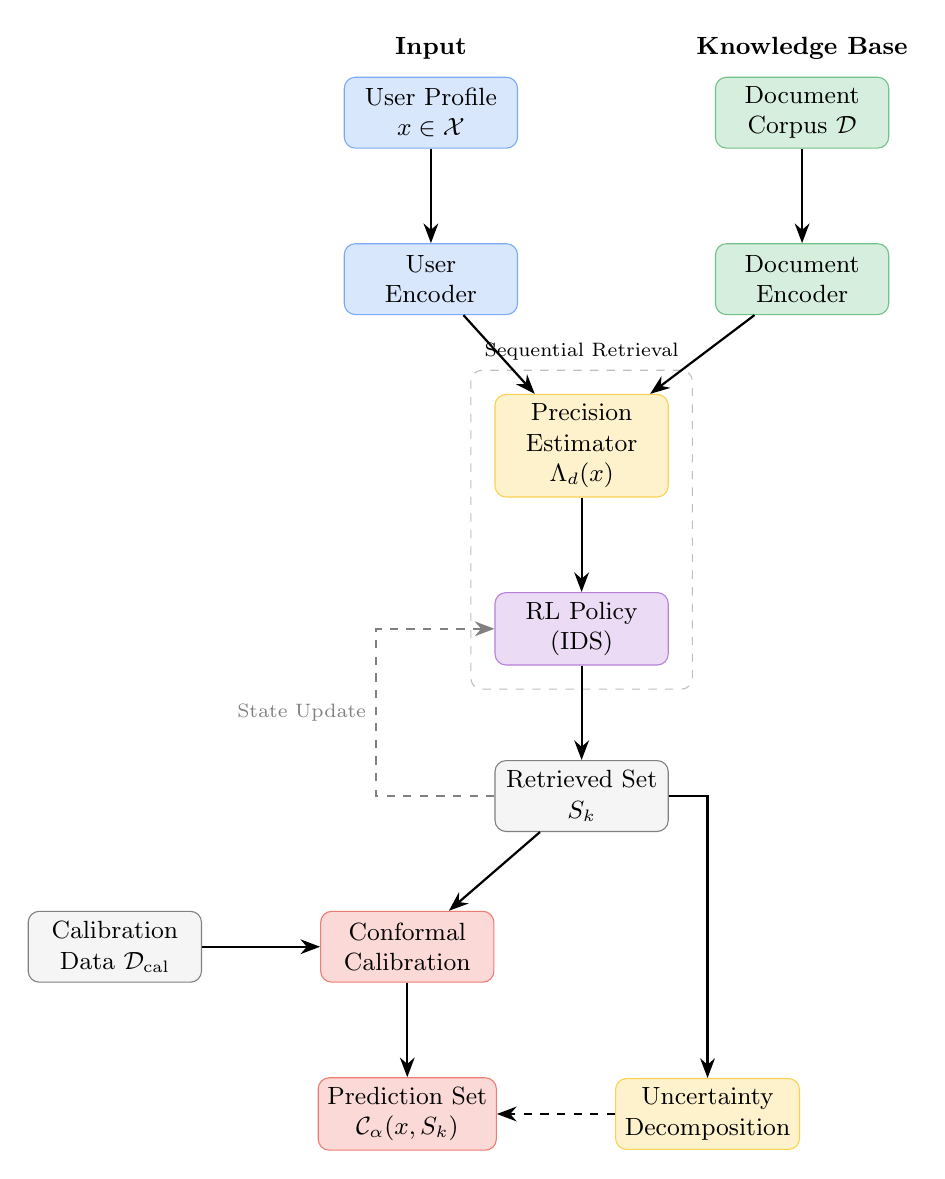
\begin{tikzpicture}[
    node distance=1.2cm and 1.5cm,
    box/.style={rectangle, draw, rounded corners, minimum width=2.2cm, minimum height=0.9cm, align=center, font=\small},
    bluebox/.style={box, fill=userblue!20, draw=userblue!70},
    greenbox/.style={box, fill=docgreen!20, draw=docgreen!70},
    orangebox/.style={box, fill=precisionorange!20, draw=precisionorange!70},
    purplebox/.style={box, fill=rlpurple!20, draw=rlpurple!70},
    redbox/.style={box, fill=conformalred!20, draw=conformalred!70},
    graybox/.style={box, fill=lightgray, draw=gray},
    arrow/.style={-{Stealth[length=2.5mm]}, thick},
    dasharrow/.style={-{Stealth[length=2.5mm]}, thick, dashed}
]

% Input layer
\node[bluebox] (profile) {User Profile\\$x \in \X$};
\node[greenbox, right=2.5cm of profile] (corpus) {Document\\Corpus $\D$};

% Encoding layer
\node[bluebox, below=of profile] (userenc) {User\\Encoder};
\node[greenbox, below=of corpus] (docenc) {Document\\Encoder};

% Precision estimation
\node[orangebox, below right=1cm and -0.3cm of userenc] (precision) {Precision\\Estimator\\$\Lambda_d(x)$};

% RL Policy
\node[purplebox, below=1.2cm of precision] (rl) {RL Policy\\(IDS)};

% Retrieved set
\node[graybox, below=of rl] (retrieved) {Retrieved Set\\$S_k$};

% Conformal calibration
\node[redbox, below left=1cm and 0cm of retrieved] (conformal) {Conformal\\Calibration};
\node[graybox, left=1.5cm of conformal] (calibdata) {Calibration\\Data $\D_{\text{cal}}$};

% Output
\node[redbox, below=of conformal] (output) {Prediction Set\\$\Ccal_\alpha(x, S_k)$};

% Uncertainty decomposition
\node[orangebox, right=1.5cm of output] (uncertainty) {Uncertainty\\Decomposition};

% Arrows
\draw[arrow] (profile) -- (userenc);
\draw[arrow] (corpus) -- (docenc);
\draw[arrow] (userenc) -- (precision);
\draw[arrow] (docenc) -- (precision);
\draw[arrow] (precision) -- (rl);
\draw[arrow] (rl) -- (retrieved);
\draw[arrow] (retrieved) -- (conformal);
\draw[arrow] (calibdata) -- (conformal);
\draw[arrow] (conformal) -- (output);
\draw[arrow] (retrieved) -| (uncertainty);
\draw[dasharrow] (uncertainty) -- (output);

% Feedback loop
\draw[dasharrow, gray] (retrieved.west) -- ++(-1.5,0) |- node[pos=0.25, left, font=\scriptsize, text=gray]{State Update} (rl.west);

% Labels
\node[above=0.1cm of profile, font=\small\bfseries] {Input};
\node[above=0.1cm of corpus, font=\small\bfseries] {Knowledge Base};

% Bounding box with title
\begin{scope}[on background layer]
    \node[draw=gray!50, dashed, rounded corners, fit=(rl)(precision), inner sep=0.3cm, label={[font=\scriptsize]above:Sequential Retrieval}] {};
\end{scope}

\end{tikzpicture}
\caption{System overview of Information-Directed Conformal Retrieval (IDCR). User profiles and documents are encoded, precision contributions are estimated, and an RL policy sequentially selects documents. The retrieved set is used for conformal calibration, producing prediction sets with coverage guarantees.}
\label{fig:system-overview}
\end{figure}

\subsection{Contributions}

This proposal presents four main contributions:

\begin{enumerate}[leftmargin=*,itemsep=0.5em]
    \item \textbf{Problem Formulation:} We formalize retrieval-augmented recommendation as a sequential decision problem where document value is measured by contribution to conformal set tightness---the first such formulation connecting retrieval to distribution-free uncertainty quantification.
    
    \item \textbf{Submodularity Result:} We prove that under a Bayesian precision aggregation model, uncertainty reduction is submodular in the retrieved document set, enabling efficient greedy optimization with provable approximation guarantees (Theorem~\ref{thm:submodularity}).
    
    \item \textbf{RL Characterization:} We introduce the document interaction tensor that precisely characterizes when reinforcement learning provides benefits over greedy retrieval (Theorem~\ref{thm:greedy-gap}), and develop an Information-Directed Sampling policy with optimal Bayesian regret bounds (Theorem~\ref{thm:ids-regret}).
    
    \item \textbf{Conformalized RL:} We prove that our RL-based retrieval policy preserves conformal coverage guarantees (Theorem~\ref{thm:coverage}), providing the first theoretical treatment of sequential retrieval under distribution-free uncertainty requirements.
\end{enumerate}

%==============================================================================
\section{Background and Preliminaries}
%==============================================================================

\subsection{Conformal Prediction}

Conformal prediction, introduced by \citet{vovk2005algorithmic}, provides a framework for constructing prediction sets with finite-sample coverage guarantees under minimal assumptions. We review the split conformal procedure, which forms the basis of our approach.

\subsubsection{Setup}

Let $\{(X_i, Y_i)\}_{i=1}^n$ be exchangeable random variables with $X_i \in \X$ and $Y_i \in \Y$. A \emph{nonconformity score function} $s: \X \times \Y \to \R$ measures how unusual a candidate output $y$ is given input $x$. Higher scores indicate greater nonconformity.

\subsubsection{Split Conformal Procedure}

Given a held-out calibration set $\{(x_i, y_i)\}_{i=1}^n$:

\begin{enumerate}[leftmargin=*]
    \item Compute calibration scores: $s_i = s(x_i, y_i)$ for $i = 1, \ldots, n$
    \item Compute the empirical quantile:
    \begin{equation}
        \hat{q} = \Quantile\left(\{s_i\}_{i=1}^n; \frac{\lceil(n+1)(1-\alpha)\rceil}{n}\right)
    \end{equation}
    \item Construct the prediction set for new input $x$:
    \begin{equation}
        \Ccal_\alpha(x) = \{y \in \Y : s(x, y) \leq \hat{q}\}
    \end{equation}
\end{enumerate}

\begin{theorem}[Vovk et al., 2005]
\label{thm:conformal-coverage}
For exchangeable calibration data and a new test point $(X_{n+1}, Y_{n+1})$, the prediction set satisfies $P(Y_{n+1} \in \Ccal_\alpha(X_{n+1})) \geq 1 - \alpha$.
\end{theorem}

The guarantee is \emph{marginal} (averaging over both calibration and test data) and \emph{distribution-free} (requiring only exchangeability, not any parametric assumptions).

\subsubsection{Efficiency and Set Volume}

While coverage is guaranteed by construction, the \emph{efficiency} of conformal prediction---measured by the size of prediction sets---depends critically on the quality of the nonconformity score and the informativeness of the conditioning set. For regression with Gaussian scores, the prediction set takes the form of an ellipsoid:
\begin{equation}
    \Ccal_\alpha(x) = \left\{y : (y - \mu(x))^\top \Sigma(x)^{-1} (y - \mu(x)) \leq \hat{q}\right\}
\end{equation}
with volume:
\begin{equation}
    \Vol(\Ccal_\alpha(x)) = \frac{\pi^{d/2}}{\Gamma(d/2 + 1)} \cdot \det(\Sigma(x))^{1/2} \cdot \hat{q}^d
\end{equation}

Minimizing set volume while maintaining coverage is the central optimization problem we address.

\subsection{Submodular Optimization}

Submodularity captures the intuitive notion of diminishing returns and enables efficient greedy optimization with provable guarantees.

\begin{definition}[Submodularity]
A set function $g: 2^V \to \R$ is \emph{submodular} if for all $A \subseteq B \subseteq V$ and $v \notin B$:
\begin{equation}
    g(A \cup \{v\}) - g(A) \geq g(B \cup \{v\}) - g(B)
\end{equation}
\end{definition}

Equivalently, the marginal gain from adding element $v$ is non-increasing as the existing set grows.

\begin{theorem}[Nemhauser et al., 1978]
\label{thm:nemhauser}
For a monotone submodular function $g$ with $g(\emptyset) = 0$, the greedy algorithm that iteratively adds the element with maximum marginal gain achieves:
\begin{equation}
    g(S_{\text{greedy}}) \geq \left(1 - \frac{1}{e}\right) \cdot g(S^*)
\end{equation}
where $S^*$ is the optimal set of size $k$.
\end{theorem}

\subsection{Information-Directed Sampling}

Information-Directed Sampling (IDS), introduced by \citet{russo2014learning}, provides a principled framework for balancing exploration and exploitation in sequential decision problems.

\subsubsection{The Information Ratio}

Let $\theta^*$ denote unknown parameters governing the reward distribution, and let $\Delta(a)$ denote the expected regret of action $a$ relative to the optimal action. The \emph{information ratio} is:
\begin{equation}
    \Psi(a) = \frac{\Delta(a)^2}{I(\theta^*; (S', R) \mid a, \Hcal_t)}
\end{equation}
where $I(\cdot; \cdot)$ denotes mutual information, $S'$ is the next state, $R$ is the reward, and $\Hcal_t$ is the history up to time $t$.

IDS selects actions minimizing the information ratio, balancing immediate regret against information gained about optimal behavior.

\begin{theorem}[Russo \& Van Roy, 2014]
\label{thm:ids-original}
Under mild regularity conditions, IDS achieves Bayesian regret $O(\sqrt{T \cdot H(\theta^*) \cdot \Psi^*})$, where $H(\theta^*)$ is the entropy of the prior over parameters and $\Psi^*$ is the worst-case information ratio.
\end{theorem}

%==============================================================================
\section{Problem Formulation}
%==============================================================================

\subsection{System Model}

We consider a retrieval-augmented recommendation system with the following components:

\begin{itemize}[leftmargin=*,itemsep=0.5em]
    \item \textbf{User Profile:} $x \in \X$ encodes observable user characteristics (risk tolerance, investment horizon, current holdings, demographic information). This is a lossy observation of the user's true latent financial state.
    
    \item \textbf{Document Corpus:} $\D = \{d_1, \ldots, d_n\}$ contains information sources (news articles, analyst reports, SEC filings, social sentiment) with embeddings $\phi(d_i) \in \R^m$.
    
    \item \textbf{Retrieved Set:} $S \subseteq \D$ with $|S| = k$ represents the documents selected for conditioning the recommendation.
    
    \item \textbf{Recommendation:} $\hat{y} = f(x, S) \in \Y$ is the system's output (portfolio weights, buy/sell signals, risk-adjusted returns).
    
    \item \textbf{Optimal Action:} $y^* \in \Y$ is the (unobserved) optimal recommendation given full information.
\end{itemize}

\subsection{Probabilistic Graphical Model}

We posit the following generative structure, visualized in Figure~\ref{fig:pgm}:
\begin{align}
    \bm{z} &\sim p(\bm{z} \mid \text{profile}) && \text{[latent user state given observed profile]} \\
    r_i &\sim p(r_i \mid \bm{z}, d_i) \in [0, 1] && \text{[relevance of document $i$ to user's latent need]} \\
    y^* &\sim p\left(y^* \,\Big|\, \bm{z}, \sum_{i=1}^{n} r_i \cdot \phi(d_i)\right) && \text{[optimal action given state + weighted documents]}
\end{align}
where $\bm{z} \in \R^k$ is a continuous latent embedding capturing the user's true financial state, preferences, and information needs.

\begin{figure}[htbp]
\centering
\begin{tikzpicture}[
    node distance=1.5cm and 2cm,
    latent/.style={circle, draw, minimum size=1.2cm, font=\small},
    observed/.style={circle, draw, minimum size=1.2cm, fill=gray!30, font=\small},
    plate/.style={draw, rectangle, rounded corners, inner sep=0.4cm},
    arrow/.style={-{Stealth[length=2.5mm]}, thick}
]

% Nodes
\node[observed] (x) {$x$};
\node[latent, right=of x] (z) {$\bm{z}$};
\node[observed, above right=0.8cm and 1.5cm of z] (d) {$d_i$};
\node[latent, right=of z] (r) {$r_i$};
\node[latent, below right=0.8cm and 1.5cm of r] (y) {$y^*$};

% Arrows
\draw[arrow] (x) -- (z);
\draw[arrow] (z) -- (r);
\draw[arrow] (d) -- (r);
\draw[arrow] (z) to[bend right=20] (y);
\draw[arrow] (r) -- (y);
\draw[arrow] (d) to[bend left=15] (y);

% Plate for documents
\node[plate, fit=(d)(r), label={[font=\scriptsize]below right:$i = 1, \ldots, n$}] {};

% Legend
\node[below=2.5cm of z, font=\small] (legend) {
    \begin{tikzpicture}
        \node[observed, minimum size=0.6cm] at (0,0) {};
        \node[right=0.3cm, font=\scriptsize] at (0.3,0) {Observed};
        \node[latent, minimum size=0.6cm] at (2.5,0) {};
        \node[right=0.3cm, font=\scriptsize] at (2.8,0) {Latent};
    \end{tikzpicture}
};

% Labels
\node[below=0.1cm of x, font=\scriptsize] {Profile};
\node[below=0.1cm of z, font=\scriptsize] {User State};
\node[above=0.1cm of d, font=\scriptsize] {Document};
\node[below=0.1cm of r, font=\scriptsize] {Relevance};
\node[below=0.1cm of y, font=\scriptsize] {Optimal Action};

\end{tikzpicture}
\caption{Probabilistic graphical model for retrieval-augmented recommendation. The observed profile $x$ generates a latent user state $\bm{z}$, which together with documents $d_i$ determines relevance scores $r_i$. The optimal recommendation $y^*$ depends on the latent state and relevance-weighted document information.}
\label{fig:pgm}
\end{figure}

\subsection{The Conformal Retrieval Objective}

We seek a retrieval policy $\pi: \X \times 2^\D \to \D$ that sequentially selects documents to minimize expected conformal set volume while maintaining coverage:
\begin{equation}
\begin{aligned}
    &\minimize_{\pi} \quad \E_x\bigl[\Vol(\Ccal_\alpha(x, S_k^\pi))\bigr] \\
    &\text{subject to} \quad P(y^* \in \Ccal_\alpha(x, S_k^\pi)) \geq 1 - \alpha
\end{aligned}
\end{equation}
where $S_k^\pi$ denotes the set of $k$ documents retrieved by policy $\pi$.

This formulation directly connects retrieval quality to downstream decision uncertainty---documents are valuable insofar as they tighten the conformal prediction set.

%==============================================================================
\section{Theoretical Framework I: Submodular Retrieval}
%==============================================================================

\subsection{Bayesian Precision Aggregation Model}

We model documents as providing precision (inverse variance) updates about the optimal recommendation. Let $\Sigma_0(x)$ denote the prior uncertainty given only the user profile. Each document $d$ contributes a positive semidefinite precision matrix $\Lambda_d(x) \succeq 0$ representing its information content for user $x$.

The posterior precision after retrieving set $S$ is:
\begin{equation}
    \Sigma(x, S)^{-1} = \Sigma_0(x)^{-1} + \sum_{d \in S} \Lambda_d(x)
\end{equation}

This is the standard Bayesian information aggregation model: each document acts as a noisy observation of $y^*$, and precisions add under conditional independence.

Figure~\ref{fig:precision-aggregation} illustrates how sequential document retrieval progressively shrinks the uncertainty ellipsoid.

\begin{figure}[htbp]
\centering
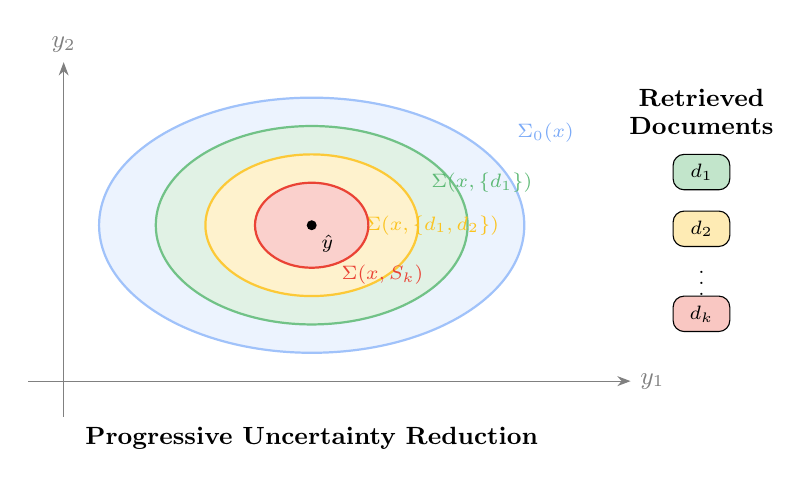
\begin{tikzpicture}[scale=0.9]
    % Axes
    \draw[-{Stealth}, gray] (-0.5,0) -- (8,0) node[right, font=\small] {$y_1$};
    \draw[-{Stealth}, gray] (0,-0.5) -- (0,4.5) node[above, font=\small] {$y_2$};
    
    % Prior ellipse (largest)
    \draw[thick, userblue!50, fill=userblue!10] (3.5,2.2) ellipse (3cm and 1.8cm);
    \node[userblue!70, font=\scriptsize] at (6.8,3.5) {$\Sigma_0(x)$};
    
    % After 1 document
    \draw[thick, docgreen!70, fill=docgreen!15] (3.5,2.2) ellipse (2.2cm and 1.4cm);
    \node[docgreen!80, font=\scriptsize] at (5.9,2.8) {$\Sigma(x, \{d_1\})$};
    
    % After 2 documents
    \draw[thick, precisionorange!80, fill=precisionorange!20] (3.5,2.2) ellipse (1.5cm and 1cm);
    \node[precisionorange!90, font=\scriptsize] at (5.2,2.2) {$\Sigma(x, \{d_1, d_2\})$};
    
    % After k documents (smallest)
    \draw[thick, conformalred, fill=conformalred!25] (3.5,2.2) ellipse (0.8cm and 0.6cm);
    \node[conformalred, font=\scriptsize] at (4.5,1.5) {$\Sigma(x, S_k)$};
    
    % True value
    \fill[black] (3.5,2.2) circle (2pt);
    \node[below right, font=\scriptsize] at (3.5,2.2) {$\hat{y}$};
    
    % Legend
    \node[font=\small\bfseries] at (3.5, -0.8) {Progressive Uncertainty Reduction};
    
    % Document icons on the side
    \begin{scope}[shift={(9,0.5)}]
        \node[font=\small\bfseries] at (0,3.5) {Retrieved};
        \node[font=\small\bfseries] at (0,3.1) {Documents};
        
        \draw[fill=docgreen!30, rounded corners] (-0.4,2.2) rectangle (0.4,2.7);
        \node[font=\scriptsize] at (0,2.45) {$d_1$};
        
        \draw[fill=precisionorange!30, rounded corners] (-0.4,1.4) rectangle (0.4,1.9);
        \node[font=\scriptsize] at (0,1.65) {$d_2$};
        
        \node[font=\scriptsize] at (0,1.0) {$\vdots$};
        
        \draw[fill=conformalred!30, rounded corners] (-0.4,0.2) rectangle (0.4,0.7);
        \node[font=\scriptsize] at (0,0.45) {$d_k$};
    \end{scope}
    
\end{tikzpicture}
\caption{Precision aggregation: Each retrieved document contributes a precision matrix $\Lambda_d(x)$, progressively shrinking the uncertainty ellipsoid (conformal prediction set) while maintaining coverage guarantees.}
\label{fig:precision-aggregation}
\end{figure}

\subsection{Uncertainty Reduction as Log-Determinant}

Define the uncertainty reduction function:
\begin{equation}
    g(S) = \log \det \Sigma_0(x) - \log \det \Sigma(x, S)
\end{equation}

This measures the reduction in differential entropy (equivalently, log-volume of the confidence ellipsoid) from retrieving documents $S$.

Applying the matrix determinant lemma:
\begin{equation}
    g(S) = \log \det\left(I + \Sigma_0(x)^{1/2} \left(\sum_{d \in S} \Lambda_d(x)\right) \Sigma_0(x)^{1/2}\right)
\end{equation}

\subsection{Submodularity Proof}

\begin{theorem}[Submodularity of Uncertainty Reduction]
\label{thm:submodularity}
The function $g(S) = \log \det \Sigma_0 - \log \det \Sigma(x, S)$ is submodular in $S$.
\end{theorem}

\begin{proof}
Define $P_d = \Sigma_0(x)^{1/2} \Lambda_d(x) \Sigma_0(x)^{1/2} \succeq 0$ and $h(M) = \log \det(I + M)$ for $M \succeq 0$. We show $h$ is concave on the PSD cone, which implies submodularity.

For the directional second derivative along direction $P \succeq 0$:
\begin{equation}
    \frac{d^2}{dt^2} h(M + tP) = \frac{d^2}{dt^2} \log \det(I + M + tP)
\end{equation}

Using the identity $\frac{\partial}{\partial t} \log \det(A + tB) = \tr((A + tB)^{-1} B)$:
\begin{align}
    \frac{d}{dt} h(M + tP) &= \tr\bigl((I + M + tP)^{-1} P\bigr) \\
    \frac{d^2}{dt^2} h(M + tP) &= -\tr\bigl((I + M + tP)^{-1} P (I + M + tP)^{-1} P\bigr)
\end{align}

Let $Q = (I + M + tP)^{-1/2} P (I + M + tP)^{-1/2}$. Then:
\begin{equation}
    \frac{d^2}{dt^2} h(M + tP) = -\tr(Q^2) = -\norm{Q}_F^2 \leq 0
\end{equation}

Thus $h$ is concave on the PSD cone.

For submodularity, consider $A \subseteq B$ and document $d \notin B$. Let $M_A = \sum_{d' \in A} P_{d'}$ and $M_B = \sum_{d' \in B} P_{d'}$. The marginal gain from adding $d$ is:
\begin{equation}
    \Delta(d \mid A) = h(M_A + P_d) - h(M_A)
\end{equation}

By concavity of $h$ and $M_A \preceq M_B$:
\begin{align}
    \Delta(d \mid A) &= \int_0^1 \tr\bigl((I + M_A + tP_d)^{-1} P_d\bigr) \, dt \\
    &\geq \int_0^1 \tr\bigl((I + M_B + tP_d)^{-1} P_d\bigr) \, dt = \Delta(d \mid B)
\end{align}

The inequality follows because $(I + M_A + tP_d)^{-1} \succeq (I + M_B + tP_d)^{-1}$ when $M_A \preceq M_B$.
\end{proof}

Figure~\ref{fig:submodularity} illustrates the diminishing returns property central to submodularity.

\begin{figure}[htbp]
\centering
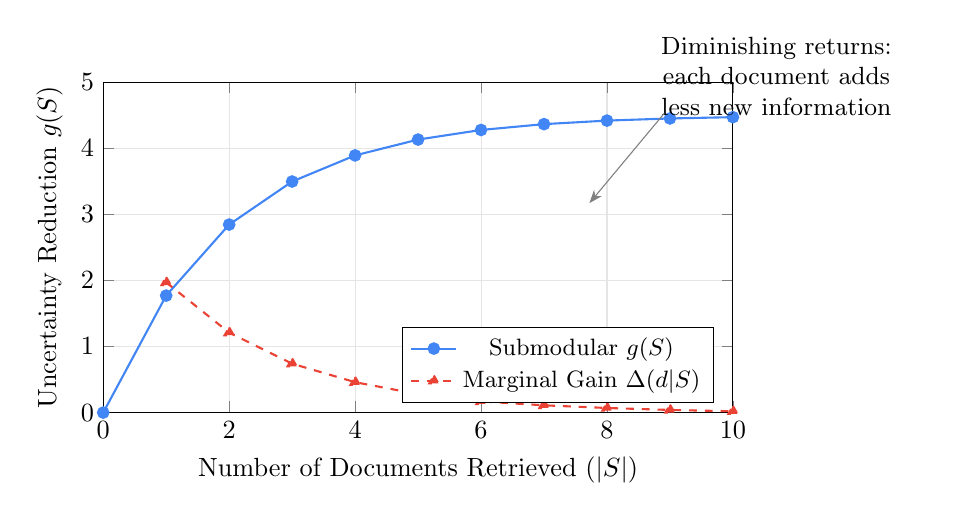
\begin{tikzpicture}[scale=0.95]
    \begin{axis}[
        width=10cm,
        height=6cm,
        xlabel={Number of Documents Retrieved ($|S|$)},
        ylabel={Uncertainty Reduction $g(S)$},
        xmin=0, xmax=10,
        ymin=0, ymax=5,
        xtick={0,2,4,6,8,10},
        ytick={0,1,2,3,4,5},
        grid=both,
        grid style={gray!20},
        legend pos=south east,
        legend style={font=\small}
    ]
    
    % Submodular curve
    \addplot[thick, userblue, mark=*, mark size=2pt, samples at={0,1,2,3,4,5,6,7,8,9,10}] 
        {4.5*(1 - exp(-0.5*x))};
    \addlegendentry{Submodular $g(S)$}
    
    % Marginal gains (decreasing)
    \addplot[thick, conformalred, dashed, mark=triangle*, mark size=2pt, samples at={1,2,3,4,5,6,7,8,9,10}] 
        coordinates {(1, 1.97) (2, 1.21) (3, 0.74) (4, 0.46) (5, 0.28) (6, 0.17) (7, 0.11) (8, 0.07) (9, 0.04) (10, 0.02)};
    \addlegendentry{Marginal Gain $\Delta(d|S)$}
    
    \end{axis}
    
    % Annotation
    \node[font=\small, text width=4cm, align=center] at (9, 4.5) {Diminishing returns:\\each document adds\\less new information};
    \draw[-{Stealth}, gray] (7.5, 4) -- (6.5, 2.8);
    
\end{tikzpicture}
\caption{Submodularity illustrated: The uncertainty reduction function $g(S)$ exhibits diminishing returns. Each additional document provides less marginal gain than the previous one, enabling efficient greedy optimization with $(1-1/e)$ approximation guarantee.}
\label{fig:submodularity}
\end{figure}

\subsection{Greedy Algorithm and Approximation Guarantee}

The submodularity result enables the following greedy algorithm:

\begin{algorithm}[H]
\caption{Greedy Conformal Retrieval}
\label{alg:greedy}
\begin{algorithmic}[1]
\Require User profile $x$, corpus $\D$, budget $k$, precision matrices $\{\Lambda_d(x)\}$
\Ensure Retrieved set $S_k$
\State $S \gets \emptyset$
\State $\Sigma_{\text{current}} \gets \Sigma_0(x)$
\For{$t = 1$ to $k$}
    \State $d^* \gets \argmax_{d \in \D \setminus S} \log \det\bigl(I + \Sigma_{\text{current}}^{1/2} \Lambda_d(x) \Sigma_{\text{current}}^{1/2}\bigr)$
    \State $S \gets S \cup \{d^*\}$
    \State $\Sigma_{\text{current}} \gets \bigl(\Sigma_{\text{current}}^{-1} + \Lambda_{d^*}(x)\bigr)^{-1}$
\EndFor
\State \Return $S$
\end{algorithmic}
\end{algorithm}

\begin{corollary}
\label{cor:greedy-approx}
The greedy algorithm achieves $g(S_{\text{greedy}}) \geq (1 - 1/e) \cdot g(S^*)$, where $S^*$ is the optimal $k$-document set.
\end{corollary}

%==============================================================================
\section{Theoretical Framework II: Reinforcement Learning}
%==============================================================================

\subsection{Limitations of Greedy Selection}

While greedy retrieval enjoys strong approximation guarantees, it is fundamentally myopic---selecting documents based only on immediate uncertainty reduction. This fails when documents exhibit \emph{complementarity}: combinations that are jointly informative but individually weak.

\subsection{Document Interaction Tensor}

We introduce a measure of higher-order document interactions that precisely characterizes when RL outperforms greedy.

\begin{definition}[Interaction Tensor]
The third-order interaction tensor $T \in \R^{n \times n \times n}$ is defined as:
\begin{align}
    T_{ijk}(x) &= I(y^*; \phi(d_i), \phi(d_j), \phi(d_k) \mid x) \nonumber \\
    &\quad - I(y^*; \phi(d_i), \phi(d_j) \mid x) - I(y^*; \phi(d_i), \phi(d_k) \mid x) - I(y^*; \phi(d_j), \phi(d_k) \mid x) \nonumber \\
    &\quad + I(y^*; \phi(d_i) \mid x) + I(y^*; \phi(d_j) \mid x) + I(y^*; \phi(d_k) \mid x)
\end{align}
\end{definition}

This is the \emph{co-information} or \emph{interaction information} among document triplets:
\begin{itemize}[leftmargin=*]
    \item $T_{ijk} > 0$: \textbf{Synergy}---documents together reveal more than sum of pairwise contributions
    \item $T_{ijk} < 0$: \textbf{Redundancy}---documents have overlapping information
    \item $T_{ijk} = 0$: No higher-order interaction
\end{itemize}

Figure~\ref{fig:synergy-redundancy} illustrates the difference between synergistic and redundant document sets.

\begin{figure}[htbp]
\centering
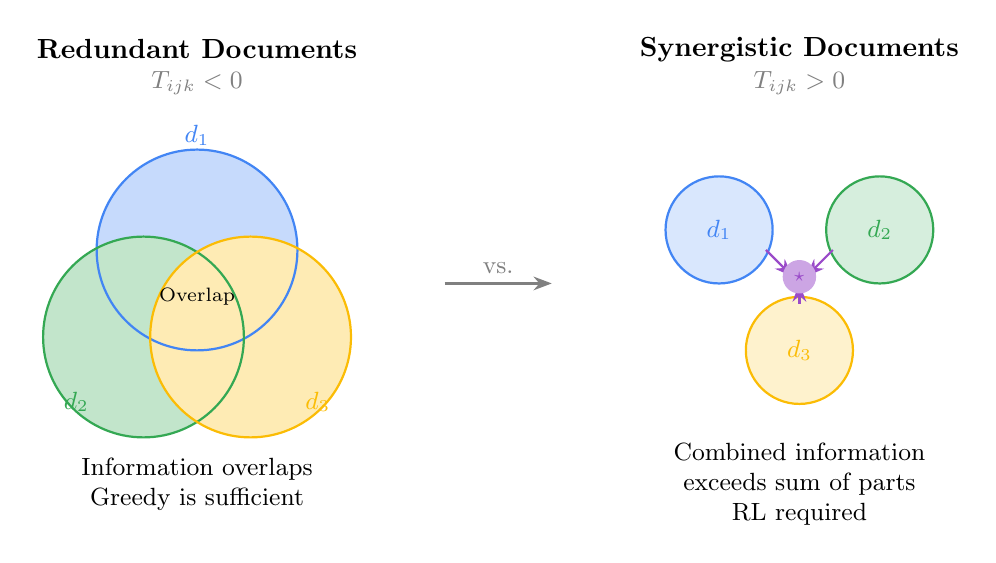
\begin{tikzpicture}[scale=0.85]
    % Left side: Redundancy
    \begin{scope}[shift={(-4.5,0)}]
        \node[font=\bfseries] at (0,3.5) {Redundant Documents};
        \node[font=\small, gray] at (0,3) {$T_{ijk} < 0$};
        
        % Three overlapping circles
        \fill[userblue!30] (0,0.5) circle (1.5cm);
        \fill[docgreen!30] (-0.8,-0.8) circle (1.5cm);
        \fill[precisionorange!30] (0.8,-0.8) circle (1.5cm);
        
        \draw[thick, userblue] (0,0.5) circle (1.5cm) node[above=1.2cm, font=\small] {$d_1$};
        \draw[thick, docgreen] (-0.8,-0.8) circle (1.5cm) node[below left=0.8cm, font=\small] {$d_2$};
        \draw[thick, precisionorange] (0.8,-0.8) circle (1.5cm) node[below right=0.8cm, font=\small] {$d_3$};
        
        % Overlap region
        \node[font=\scriptsize] at (0,-0.2) {Overlap};
        
        \node[font=\small, text width=3.5cm, align=center] at (0,-3) {Information overlaps\\Greedy is sufficient};
    \end{scope}
    
    % Right side: Synergy
    \begin{scope}[shift={(4.5,0)}]
        \node[font=\bfseries] at (0,3.5) {Synergistic Documents};
        \node[font=\small, gray] at (0,3) {$T_{ijk} > 0$};
        
        % Three separate circles
        \draw[thick, userblue, fill=userblue!20] (-1.2,0.8) circle (0.8cm) node[font=\small] {$d_1$};
        \draw[thick, docgreen, fill=docgreen!20] (1.2,0.8) circle (0.8cm) node[font=\small] {$d_2$};
        \draw[thick, precisionorange, fill=precisionorange!20] (0,-1) circle (0.8cm) node[font=\small] {$d_3$};
        
        % Synergy arrows pointing to center
        \draw[-{Stealth}, thick, rlpurple] (-0.5,0.5) -- (-0.1,0.1);
        \draw[-{Stealth}, thick, rlpurple] (0.5,0.5) -- (0.1,0.1);
        \draw[-{Stealth}, thick, rlpurple] (0,-0.3) -- (0,0);
        
        % Central synergy
        \fill[rlpurple!50] (0,0.1) circle (0.25cm);
        \node[font=\scriptsize, rlpurple] at (0,0.1) {$\star$};
        
        \node[font=\small, text width=3.5cm, align=center] at (0,-3) {Combined information\\exceeds sum of parts\\RL required};
    \end{scope}
    
    % Comparison arrow
    \draw[thick, gray, -{Stealth}] (-0.8,0) -- (0.8,0);
    \node[font=\small, gray, above] at (0,0) {vs.};
    
\end{tikzpicture}
\caption{Redundancy vs. Synergy in document sets. Left: Redundant documents have overlapping information ($T_{ijk} < 0$); greedy retrieval is optimal. Right: Synergistic documents together reveal information unavailable from any subset ($T_{ijk} > 0$); RL can exploit complementarity for better performance.}
\label{fig:synergy-redundancy}
\end{figure}

\begin{theorem}[Greedy Suboptimality Characterization]
\label{thm:greedy-gap}
Let $\Delta_k = V^{\pi^*}(s_0) - V^{\pi_{\text{greedy}}}(s_0)$ denote the value gap between optimal and greedy policies. Then:
\begin{equation}
    \Delta_k \leq k \cdot \max_{i,j,\ell} \abs{T_{ij\ell}(x)} \cdot \ind[\exists \text{ positive synergy}]
\end{equation}
Consequently, if all document interactions are purely redundant ($T_{ijk} \leq 0$ for all $i,j,k$), greedy is optimal.
\end{theorem}

This theorem provides a \emph{testable condition}: RL benefits exist if and only if synergistic document combinations exist.

\subsection{MDP Formulation}

We formalize sequential retrieval as a finite-horizon Markov Decision Process, illustrated in Figure~\ref{fig:mdp}:

\begin{itemize}[leftmargin=*,itemsep=0.5em]
    \item \textbf{State:} $s_t = (x, S_t, k-t) \in \X \times 2^\D \times \N$, comprising user profile, retrieved documents, and remaining budget
    
    \item \textbf{Action:} $a_t \in \D \setminus S_t$, selecting one document from the remaining corpus
    
    \item \textbf{Transition:} $s_{t+1} = (x, S_t \cup \{a_t\}, k-t-1)$, deterministic
    
    \item \textbf{Reward:} $r_t = I(y^*; \phi(a_t) \mid x, S_t)$, the conditional mutual information between the selected document and optimal recommendation
    
    \item \textbf{Terminal Value:} $V(s_k) = -\log \det \Sigma(x, S_k)$, the negative log-volume of the conformal ellipsoid
\end{itemize}

\begin{figure}[htbp]
\centering
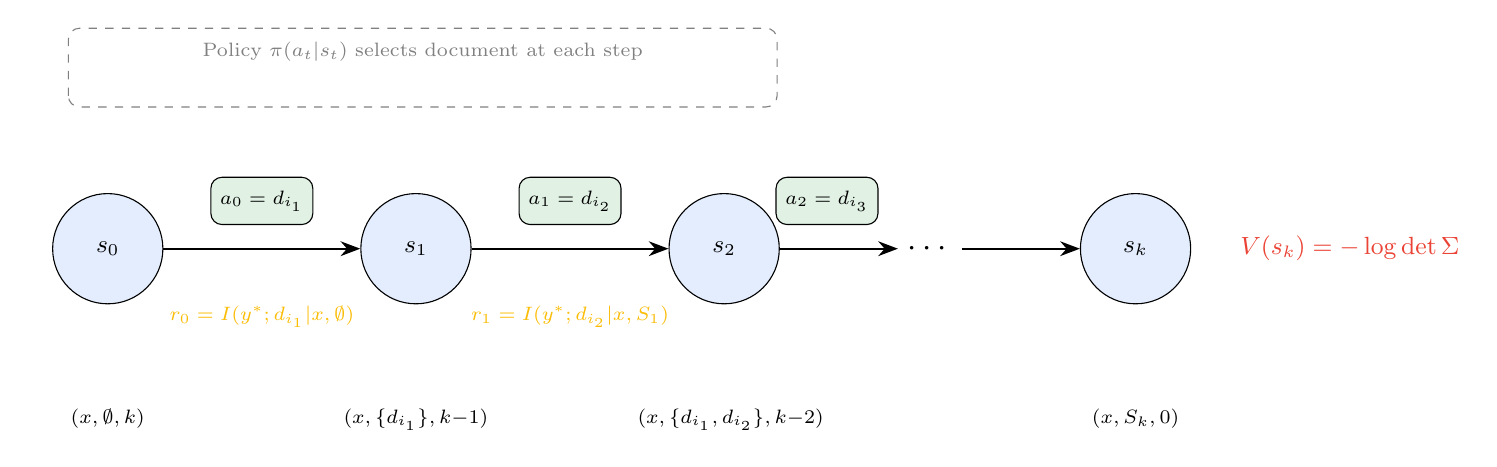
\begin{tikzpicture}[
    node distance=2.5cm,
    state/.style={circle, draw, minimum size=1.4cm, font=\small, fill=userblue!15},
    action/.style={rectangle, draw, rounded corners, minimum width=1cm, minimum height=0.6cm, font=\scriptsize, fill=docgreen!15},
    reward/.style={font=\scriptsize, precisionorange},
    arrow/.style={-{Stealth[length=2.5mm]}, thick}
]

% States
\node[state] (s0) {$s_0$};
\node[state, right=of s0] (s1) {$s_1$};
\node[state, right=of s1] (s2) {$s_2$};
\node[right=1.5cm of s2, font=\large] (dots) {$\cdots$};
\node[state, right=1.5cm of dots] (sk) {$s_k$};

% Actions (above arrows)
\node[action, above=0.3cm of $(s0)!0.5!(s1)$] (a0) {$a_0 = d_{i_1}$};
\node[action, above=0.3cm of $(s1)!0.5!(s2)$] (a1) {$a_1 = d_{i_2}$};
\node[action, above=0.3cm of $(s2)!0.5!(dots)$] (a2) {$a_2 = d_{i_3}$};

% Arrows between states
\draw[arrow] (s0) -- (s1);
\draw[arrow] (s1) -- (s2);
\draw[arrow] (s2) -- (dots);
\draw[arrow] (dots) -- (sk);

% Rewards (below arrows)
\node[reward, below=0.6cm of $(s0)!0.5!(s1)$] {$r_0 = I(y^*; d_{i_1} | x, \emptyset)$};
\node[reward, below=0.6cm of $(s1)!0.5!(s2)$] {$r_1 = I(y^*; d_{i_2} | x, S_1)$};

% State descriptions
\node[below=1.2cm of s0, font=\scriptsize, text width=1.8cm, align=center] {$(x, \emptyset, k)$};
\node[below=1.2cm of s1, font=\scriptsize, text width=2cm, align=center] {$(x, \{d_{i_1}\}, k{-}1)$};
\node[below=1.2cm of s2, font=\scriptsize, text width=2.2cm, align=center] {$(x, \{d_{i_1}, d_{i_2}\}, k{-}2)$};
\node[below=1.2cm of sk, font=\scriptsize, text width=2cm, align=center] {$(x, S_k, 0)$};

% Terminal value
\node[right=0.5cm of sk, font=\small, conformalred] {$V(s_k) = -\log\det\Sigma$};

% Policy annotation
\draw[dashed, gray, rounded corners] (-0.5,1.8) rectangle (8.5,2.8);
\node[font=\scriptsize, gray] at (4, 2.5) {Policy $\pi(a_t | s_t)$ selects document at each step};

\end{tikzpicture}
\caption{MDP formulation for sequential document retrieval. States encode the user profile, retrieved set, and remaining budget. Actions select documents, and rewards measure information gain. The terminal value is the negative log-volume of the uncertainty ellipsoid.}
\label{fig:mdp}
\end{figure}

\subsection{Information-Directed Sampling for Retrieval}

We adapt IDS to the retrieval setting. The key insight is that early retrievals should \emph{explore} to learn which documents are informative for this user, while later retrievals should \emph{exploit} the learned model.

Let $\theta = \{\Lambda_d(x)\}_{d \in \D}$ denote the precision contribution parameters. The IDS action selection is:
\begin{equation}
    a_t^{\text{IDS}} = \argmin_{a \in \D \setminus S_t} \Psi(a)
\end{equation}
where the information ratio is:
\begin{equation}
    \Psi(a) = \frac{\bigl(\Delta_{\text{greedy}}(a)\bigr)^2}{I\bigl(\theta; \Sigma(x, S_t \cup \{a\}) \mid \Hcal_t\bigr)}
\end{equation}

Here $\Delta_{\text{greedy}}(a) = r(s_t, a^*_{\text{greedy}}) - r(s_t, a)$ is the immediate regret relative to the greedy choice, and the denominator is the information gained about the precision parameters.

\begin{theorem}[IDS Regret Bound]
\label{thm:ids-regret}
For the conformal retrieval MDP with IDS policy:
\begin{equation}
    \text{BayesRegret}(T, \pi^{\text{IDS}}) \leq \sqrt{2T \cdot H(\theta^*) \cdot \Psi^*}
\end{equation}
where $H(\theta^*)$ is the entropy of the prior over precision parameters and $\Psi^*$ is the worst-case information ratio. This achieves the optimal $\tilde{O}(\sqrt{T})$ rate.
\end{theorem}

\subsection{Preservation of Conformal Coverage}

A critical concern is whether the RL policy, which adapts based on training data, preserves the distribution-free coverage guarantee.

\begin{theorem}[Coverage Preservation]
\label{thm:coverage}
Let $\pi_\phi$ be an RL policy trained on dataset $\D_{\text{train}}$. If calibration is performed on a held-out set $\D_{\text{cal}}$ independent of $\D_{\text{train}}$, then for any test point $(x, y^*)$:
\begin{equation}
    P\bigl(y^* \in \Ccal_\alpha(x, S_k^{\pi_\phi})\bigr) \geq 1 - \alpha
\end{equation}
\end{theorem}

\begin{proof}
The conformal guarantee requires only exchangeability of calibration points. Since $\D_{\text{cal}} \perp\!\!\!\perp \D_{\text{train}}$, exchangeability holds. The policy $\pi_\phi$ is fixed at calibration time---it is a deterministic function of $\D_{\text{train}}$. Thus $S_k^{\pi_\phi}(x)$ is a deterministic function of $x$ (given fixed $\pi_\phi$), and the standard split conformal guarantee applies.
\end{proof}

\begin{theorem}[Efficiency-Quality Relationship]
\label{thm:efficiency}
Let $\pi_1, \pi_2$ be two retrieval policies with $V^{\pi_1}(s_0) > V^{\pi_2}(s_0)$ ($\pi_2$ achieves lower uncertainty). Then the conformal set volumes satisfy:
\begin{equation}
    \E\bigl[\Vol(\Ccal_\alpha^{\pi_2})\bigr] \leq \E\bigl[\Vol(\Ccal_\alpha^{\pi_1})\bigr]
\end{equation}
Better retrieval policies yield tighter prediction sets.
\end{theorem}

%==============================================================================
\section{Learning Framework}
%==============================================================================

\subsection{Precision Predictor Architecture}

The theoretical framework assumes access to precision matrices $\Lambda_d(x)$. In practice, these are learned from data. The architecture is shown in Figure~\ref{fig:architecture}.

\begin{figure}[htbp]
\centering
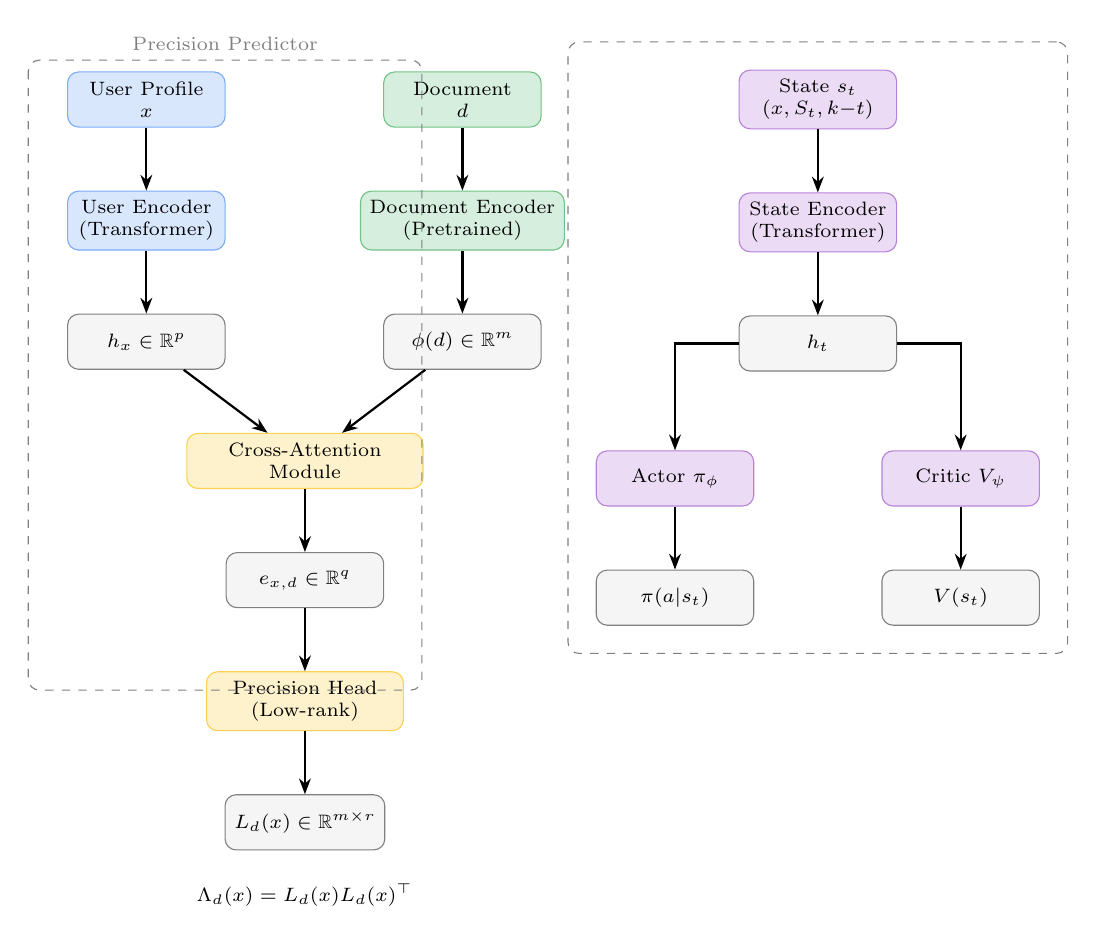
\begin{tikzpicture}[
    node distance=0.8cm and 1.2cm,
    box/.style={rectangle, draw, rounded corners, minimum width=2cm, minimum height=0.7cm, align=center, font=\scriptsize},
    bluebox/.style={box, fill=userblue!20, draw=userblue!70},
    greenbox/.style={box, fill=docgreen!20, draw=docgreen!70},
    orangebox/.style={box, fill=precisionorange!20, draw=precisionorange!70},
    purplebox/.style={box, fill=rlpurple!20, draw=rlpurple!70},
    graybox/.style={box, fill=lightgray, draw=gray},
    arrow/.style={-{Stealth[length=2mm]}, thick},
    label/.style={font=\scriptsize, gray}
]

% Input layer
\node[bluebox] (profile) {User Profile\\$x$};
\node[greenbox, right=2cm of profile] (doc) {Document\\$d$};

% Encoders
\node[bluebox, below=of profile] (userenc) {User Encoder\\(Transformer)};
\node[greenbox, below=of doc] (docenc) {Document Encoder\\(Pretrained)};

% Representations
\node[graybox, below=of userenc] (hx) {$h_x \in \R^p$};
\node[graybox, below=of docenc] (phid) {$\phi(d) \in \R^m$};

% Cross attention
\node[orangebox, below right=0.8cm and -0.5cm of hx, minimum width=3cm] (cross) {Cross-Attention\\Module};

% Interaction
\node[graybox, below=of cross] (exd) {$e_{x,d} \in \R^q$};

% Precision head
\node[orangebox, below=of exd, minimum width=2.5cm] (prechead) {Precision Head\\(Low-rank)};

% Output
\node[graybox, below=of prechead] (lambda) {$L_d(x) \in \R^{m \times r}$};
\node[below=0.3cm of lambda, font=\scriptsize] {$\Lambda_d(x) = L_d(x)L_d(x)^\top$};

% Arrows
\draw[arrow] (profile) -- (userenc);
\draw[arrow] (doc) -- (docenc);
\draw[arrow] (userenc) -- (hx);
\draw[arrow] (docenc) -- (phid);
\draw[arrow] (hx) -- (cross);
\draw[arrow] (phid) -- (cross);
\draw[arrow] (cross) -- (exd);
\draw[arrow] (exd) -- (prechead);
\draw[arrow] (prechead) -- (lambda);

% Add \usetikzlibrary{fit} to your preamble

% Actor-Critic Section (Anchored to the right of the document column)
\node[purplebox, right=2.5cm of doc] (state) {State $s_t$\\$(x, S_t, k{-}t)$};

\node[purplebox, below=of state] (stateenc) {State Encoder\\(Transformer)};
\node[graybox, below=of stateenc] (ht) {$h_t$};

% Split Actor and Critic
\node[purplebox, below left=1cm and -0.2cm of ht] (actor) {Actor $\pi_\phi$};
\node[purplebox, below right=1cm and -0.2cm of ht] (critic) {Critic $V_\psi$};

\node[graybox, below=0.8cm of actor] (policy) {$\pi(a|s_t)$};
\node[graybox, below=0.8cm of critic] (value) {$V(s_t)$};

% Arrows for Actor-Critic
\draw[arrow] (state) -- (stateenc);
\draw[arrow] (stateenc) -- (ht);
\draw[arrow] (ht) -| (actor);
\draw[arrow] (ht) -| (critic);
\draw[arrow] (actor) -- (policy);
\draw[arrow] (critic) -- (value);

% % Dashed Containers using the 'fit' library
% \node[draw, dashed, gray, rounded corners, inner sep=10pt, 
%       fit=(profile) (userenc) (hx) (lambda), 
%       label={[gray, font=\scriptsize]above:Precision Predictor}] (box1) {};

\node[draw, dashed, gray, rounded corners, inner sep=10pt, 
      fit=(state) (stateenc) (policy) (value), 
      label={[gray, font=\scriptsize]above:RL Policy}] (box2) {};

% Connecting box
\draw[dashed, gray, rounded corners] (-1.5,0.5) rectangle (3.5,-7.5);
\node[font=\scriptsize, gray, above] at (1, 0.5) {Precision Predictor};

% \draw[dashed, gray, rounded corners] (4.5,0.5) rectangle (8,-7.5);
% \node[font=\scriptsize, gray, above] at (6.25, 0.5) {RL Policy};

\end{tikzpicture}
\caption{Neural network architecture for IDCR. Left: Precision predictor estimates $\Lambda_d(x)$ via user-document cross-attention and low-rank factorization. Right: Actor-critic architecture for sequential retrieval with state encoding, policy network, and value network.}
\label{fig:architecture}
\end{figure}

\textbf{Architecture components:}
\begin{enumerate}[leftmargin=*]
    \item \textbf{User Encoder:} A transformer network mapping profile $x$ to latent representation $h_x \in \R^p$
    
    \item \textbf{Document Encoder:} A pretrained or fine-tuned embedder producing $\phi(d) \in \R^m$
    
    \item \textbf{Cross-Attention Module:} Computing user-document interaction $e_{x,d} \in \R^q$ via attention between $h_x$ and $\phi(d)$
    
    \item \textbf{Precision Head:} A low-rank factorization $L_d(x) \in \R^{m \times r}$ such that $\Lambda_d(x) = L_d(x) L_d(x)^\top$, ensuring positive semidefiniteness
\end{enumerate}

\subsection{Training Objectives}

The precision predictor is trained with a composite objective:

\subsubsection{Calibration Loss (Coverage)}

The prediction sets must achieve valid coverage:
\begin{equation}
    \Lcal_{\text{coverage}} = \left(\frac{1}{n}\sum_{i=1}^n \ind[y_i \notin \Ccal_\alpha(x_i, S_i)] - \alpha\right)^2
\end{equation}

\subsubsection{Efficiency Loss (Set Size)}

Smaller sets are preferred, conditional on valid coverage:
\begin{equation}
    \Lcal_{\text{efficiency}} = \frac{1}{n}\sum_{i=1}^n \log \det \Sigma_\theta(x_i, S_i)
\end{equation}

\subsubsection{Ranking Consistency Loss (Self-Supervised)}

Documents ranked higher should contribute more precision:
\begin{equation}
    \Lcal_{\text{rank}} = \sum_{\substack{(d, d'): \\ \text{rank}(d) < \text{rank}(d')}} \max\bigl(0, \tr(\Lambda_{d'}(x)) - \tr(\Lambda_d(x)) + \gamma\bigr)
\end{equation}

\textbf{Total objective:}
\begin{equation}
    \Lcal = \Lcal_{\text{efficiency}} + \lambda_1 \Lcal_{\text{coverage}} + \lambda_2 \Lcal_{\text{rank}}
\end{equation}

\subsection{Actor-Critic Training}

Policy gradient with information-directed regularization:
\begin{equation}
    \Lcal_{\text{actor}} = -\E_{\tau \sim \pi_\phi}\left[\sum_t \bigl(r_t + \lambda b_t(a_t) - V_\psi(s_t)\bigr) \log \pi_\phi(a_t \mid s_t)\right]
\end{equation}

where $b_t(a) = \hat{I}(\theta; \Sigma(x, S_t \cup \{a\}) \mid \Hcal_t)$ is the information bonus estimated via ensemble disagreement.

%==============================================================================
\section{Uncertainty Decomposition}
%==============================================================================

The framework provides three interpretable uncertainty components, visualized in Figure~\ref{fig:% Replace your Reducible brace with this:
\draw[decorate, decoration={brace, amplitude=8pt, mirror}, thick, gray] 
    ([yshift=-1.4cm]user.south west) -- ([yshift=-1.4cm]doc.south east) 
    node[midway, below=0.4cm, font=\scriptsize, gray, align=center] {Reducible\\(better retrieval / more profile data)};

% Replace your Irreducible brace with this:
\draw[decorate, decoration={brace, amplitude=8pt, mirror}, thick, gray] 
    ([yshift=-1.4cm]irreducible.south west) -- ([yshift=-1.4cm]irreducible.south east) 
    node[midway, below=0.4cm, font=\scriptsize, gray] {Irreducible};}:

\begin{figure}[htbp]
\centering
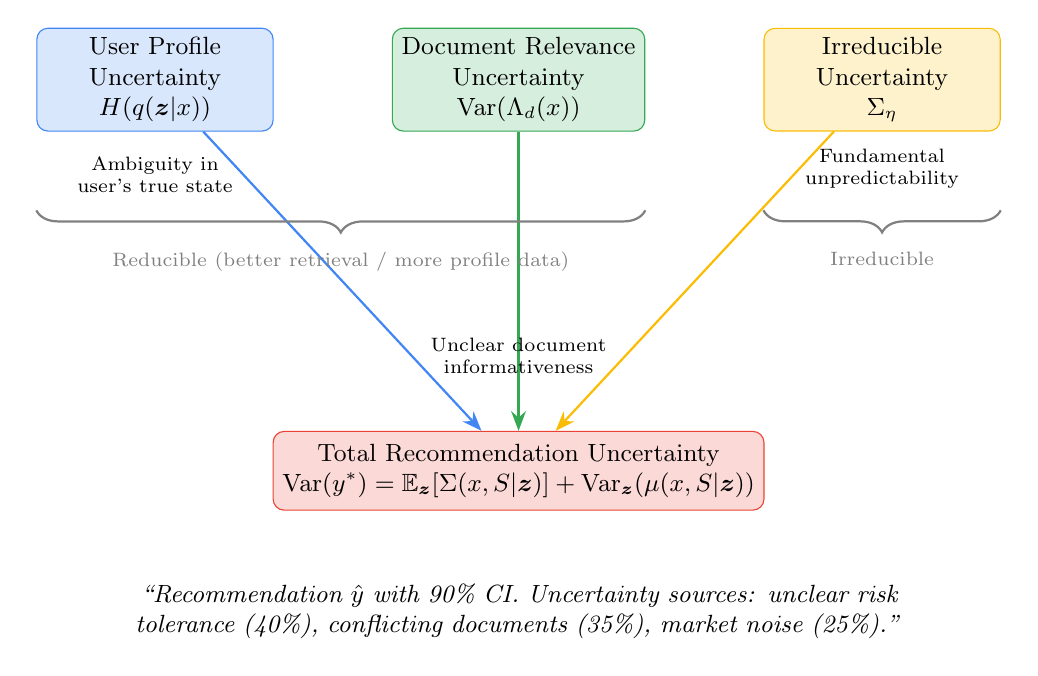
\begin{tikzpicture}[
    node distance=1cm,
    box/.style={rectangle, draw, rounded corners, minimum width=3cm, minimum height=1cm, align=center, font=\small},
    arrow/.style={-{Stealth[length=2.5mm]}, thick}
]

% Main components
\node[box, fill=userblue!20, draw=userblue] (user) {User Profile\\Uncertainty\\$H(q(\bm{z}|x))$};

\node[box, fill=docgreen!20, draw=docgreen, right=1.5cm of user] (doc) {Document Relevance\\Uncertainty\\$\Var(\Lambda_d(x))$};

\node[box, fill=precisionorange!20, draw=precisionorange, right=1.5cm of doc] (irreducible) {Irreducible\\Uncertainty\\$\Sigma_\eta$};

% Combination
\node[box, fill=conformalred!20, draw=conformalred, below=3.8cm of doc, minimum width=5cm] (total) {Total Recommendation Uncertainty\\$\Var(y^*) = \E_{\bm{z}}[\Sigma(x,S|\bm{z})] + \Var_{\bm{z}}(\mu(x,S|\bm{z}))$};

% Arrows
\draw[arrow, userblue] (user) -- (total);
\draw[arrow, docgreen] (doc) -- (total);
\draw[arrow, precisionorange] (irreducible) -- (total);

% Labels
\node[below=0.2cm of user, font=\scriptsize, text width=3cm, align=center] {Ambiguity in\\user's true state};
\node[below=2.5cm of doc, font=\scriptsize, text width=3cm, align=center] {Unclear document\\informativeness};
\node[below=0.1cm of irreducible, font=\scriptsize, text width=3cm, align=center] {Fundamental\\unpredictability};

% Output annotation
\node[below=0.8cm of total, font=\small, text width=10cm, align=center] {
    \textit{``Recommendation $\hat{y}$ with 90\% CI. Uncertainty sources: unclear risk tolerance (40\%), conflicting documents (35\%), market noise (25\%).''}
};

% Reducible vs irreducible
\draw[decorate, decoration={brace, amplitude=8pt, mirror}, thick, gray] 
    ([yshift=-1cm]user.south west) -- ([yshift=-1cm]doc.south east) node[midway, below=0.4cm, font=\scriptsize, gray] {Reducible (better retrieval / more profile data)};
    
\draw[decorate, decoration={brace, amplitude=8pt, mirror}, thick, gray] 
    ([yshift=-1cm]irreducible.south west) -- ([yshift=-1cm]irreducible.south east) node[midway, below=0.4cm, font=\scriptsize, gray] {Irreducible};

\end{tikzpicture}
\caption{Uncertainty decomposition in IDCR. Total recommendation uncertainty decomposes into three interpretable components: user profile ambiguity, document relevance uncertainty, and irreducible noise. The first two can be reduced through better retrieval or additional profile information.}
\label{fig:uncertainty-decomposition}
\end{figure}

\subsection{User Profile Uncertainty}
\begin{equation}
    H_{\text{user}} = H(q(\bm{z} \mid \text{profile}))
\end{equation}
High when the profile is ambiguous about the user's true latent state. \emph{Example:} insufficient trading history to determine risk tolerance.

\subsection{Document Relevance Uncertainty}
\begin{equation}
    H_{\text{doc}}(d) = \Var_q(r_d) = \Var(\Lambda_d(x))
\end{equation}
High for documents whose informativeness is unclear. \emph{Example:} an analyst report covering multiple sectors when user exposure is uncertain.

\subsection{Recommendation Uncertainty}

The total recommendation uncertainty propagates both sources:
\begin{equation}
    \Var(y^*) = \E_{\bm{z}}\bigl[\Sigma(x, S \mid \bm{z})\bigr] + \Var_{\bm{z}}\bigl(\mu(x, S \mid \bm{z})\bigr)
\end{equation}

This is an application of the law of total variance, decomposing into expected conditional variance (irreducible given $\bm{z}$) plus variance of conditional means (reducible by resolving user uncertainty).

%==============================================================================
\section{Experimental Design}
%==============================================================================

\subsection{Synthetic Data Generation}

We construct a synthetic environment with controlled properties to validate theoretical predictions:

\subsubsection{User Profiles}

Sample from a mixture of $K$ archetypal investor profiles (conservative retiree, aggressive trader, balanced investor, etc.) with continuous interpolation:
\begin{equation}
    x \sim \sum_{k=1}^K w_k \, \mathcal{N}(\mu_k, \Sigma_k)
\end{equation}
Profile dimensions encode: risk tolerance, investment horizon, sector exposure preferences, liquidity needs.

\subsubsection{Documents with Known Precision}

Generate documents with ground-truth precision contributions $\Lambda_d^*(x)$. For each document:
\begin{itemize}[leftmargin=*]
    \item Sample an informativeness level $\lambda_d \sim \text{Gamma}(\alpha, \beta)$
    \item Sample user-type specificity (which archetypes it informs)
    \item Construct $\Lambda_d^*(x) = \lambda_d \cdot P_d(x)$ where $P_d(x)$ projects onto relevant dimensions
\end{itemize}

\subsubsection{Controlled Synergy Structure}

To test the RL vs.\ greedy characterization, create document sets with known interaction properties:
\begin{itemize}[leftmargin=*]
    \item \textbf{Redundant corpus:} All documents provide overlapping information ($T_{ijk} < 0$)
    \item \textbf{Synergistic corpus:} Specific pairs/triples unlock new information ($T_{ijk} > 0$)
    \item \textbf{Mixed corpus:} Realistic combination
\end{itemize}

\subsection{Experiments}

\begin{enumerate}[leftmargin=*,label=\textbf{Experiment \arabic*:},itemsep=1em]
    \item \textbf{Submodularity Verification} \\
    Empirically verify diminishing returns by computing marginal gains $\Delta(d \mid S)$ for varying $|S|$. \\
    \emph{Hypothesis:} $\Delta(d \mid S)$ is non-increasing in $|S|$.
    
    \item \textbf{Greedy Approximation Quality} \\
    Compare greedy retrieval to optimal (computed via enumeration for small $k$) on varying corpus structures. \\
    \emph{Hypothesis:} Greedy achieves $\geq 63\%$ of optimal uncertainty reduction across all settings.
    
    \item \textbf{RL vs.\ Greedy under Synergy} \\
    Train RL policy on synergistic, redundant, and mixed corpora. Compare to greedy baseline. \\
    \emph{Hypothesis:} RL outperforms greedy on synergistic/mixed corpora; matches greedy on redundant corpus.
    
    \item \textbf{Interaction Tensor Prediction} \\
    Estimate $T_{ijk}$ from data. Verify correlation between positive synergy and RL improvement. \\
    \emph{Hypothesis:} Estimated synergy predicts RL benefit magnitude.
    
    \item \textbf{Coverage Verification} \\
    Verify distribution-free coverage guarantee across retrieval policies (random, greedy, RL). \\
    \emph{Hypothesis:} All policies achieve $\geq (1-\alpha)$ coverage; RL achieves smallest set volume.
    
    \item \textbf{Efficiency-Coverage Pareto} \\
    Plot (coverage rate, set volume) Pareto frontier for varying $\alpha$ and retrieval budget $k$. \\
    \emph{Hypothesis:} RL dominates other policies (achieves same coverage with smaller sets).
\end{enumerate}

%==============================================================================
\section{Implementation Timeline}
%==============================================================================

\begin{table}[h]
\centering
\begin{tabular}{@{}lp{10cm}@{}}
\toprule
\textbf{Week} & \textbf{Deliverables} \\
\midrule
Week 1 & \textbf{Foundation:} Implement split conformal prediction for base recommender. Synthetic data generation pipeline with controlled precision contributions. Verify empirical coverage. Implement ellipsoidal set volume computation. \\[1em]
Week 2 & \textbf{Core Algorithm:} Precision predictor network (user encoder + cross-attention + precision head). Greedy retrieval algorithm with submodularity verification. Training loop with composite loss function. \\[1em]
Week 3 & \textbf{RL Integration:} Actor-critic implementation with information bonus. IDS objective and information ratio computation. Synthetic corpora with controlled synergy structure. Interaction tensor estimation. \\[1em]
Week 4 & \textbf{Experiments and Documentation:} Complete experimental suite (6 experiments). Generate figures and analysis. Final documentation and technical report. Code cleanup and reproducibility verification. \\
\bottomrule
\end{tabular}
\end{table}

%==============================================================================
\section{Summary of Theoretical Contributions}
%==============================================================================

\begin{table}[h]
\centering
\begin{tabular}{@{}lp{9cm}@{}}
\toprule
\textbf{Contribution} & \textbf{Description} \\
\midrule
Problem Formulation & First formalization of retrieval as conformal set minimization, connecting information retrieval, uncertainty quantification, and decision theory. \\[0.5em]
Theorem~\ref{thm:submodularity} & Submodularity of log-determinant uncertainty reduction under Bayesian precision aggregation, enabling greedy retrieval with $(1-1/e)$ approximation guarantee. \\[0.5em]
Theorem~\ref{thm:greedy-gap} & Interaction tensor characterization of when RL outperforms greedy retrieval. Provides testable condition: RL benefits exist iff synergistic document combinations exist. \\[0.5em]
Theorem~\ref{thm:ids-regret} & Optimal $\tilde{O}(\sqrt{T})$ Bayesian regret bound for IDS policy in the retrieval MDP, with explicit dependence on document synergy structure. \\[0.5em]
Theorem~\ref{thm:coverage} & Conformalized RL: Proof that RL-based retrieval preserves distribution-free coverage guarantees under train/calibration data independence. \\[0.5em]
Theorem~\ref{thm:efficiency} & Quantitative relationship between policy quality (value function) and conformal set efficiency (volume). Better retrieval $\Rightarrow$ tighter uncertainty bounds. \\
\bottomrule
\end{tabular}
\end{table}

%==============================================================================
\newpage
\appendix
\section{Complete Algorithm}
%==============================================================================

\begin{algorithm}[H]
\caption{Information-Directed Conformal Retrieval (IDCR) --- Full Procedure}
\label{alg:idcr-full}
\begin{algorithmic}[1]
\Require User profile $x$, corpus $\D$, budget $k$, trained networks $(\pi_\phi, V_\psi, \Lambda_\theta)$
\Require Calibration set $\D_{\text{cal}}$, confidence level $\alpha$
\Ensure Retrieved set $S_k$, prediction set $\Ccal_\alpha$, uncertainty decomposition

\Statex
\Statex \textbf{Phase 1: Sequential Retrieval}
\State $S_0 \gets \emptyset$
\State $\Sigma_{\text{current}} \gets \Sigma_0(x)$ \Comment{Prior uncertainty}

\For{$t = 0$ to $k-1$}
    \State $h_t \gets \text{StateEncoder}(x, S_t)$ \Comment{Compute state representation}
    
    \For{$d \in \D \setminus S_t$} \Comment{Score all candidates}
        \State $q_{\text{exploit}}(d) \gets \log \det\bigl(I + \Sigma_{\text{current}}^{1/2} \Lambda_\theta(d,x) \Sigma_{\text{current}}^{1/2}\bigr)$ \Comment{Exploitation}
        \State $q_{\text{explore}}(d) \gets \text{EnsembleDisagreement}(\Lambda_\theta(d, x))$ \Comment{Exploration}
        \State $q(d) \gets q_{\text{exploit}}(d) + \lambda_t \cdot q_{\text{explore}}(d)$ \Comment{IDS objective}
    \EndFor
    
    \State $a_t \gets \argmax_d q(d)$ \Comment{Select best document}
    \State $S_{t+1} \gets S_t \cup \{a_t\}$
    \State $\Sigma_{\text{current}} \gets \bigl(\Sigma_{\text{current}}^{-1} + \Lambda_\theta(a_t, x)\bigr)^{-1}$ \Comment{Update posterior}
\EndFor

\Statex
\Statex \textbf{Phase 2: Conformal Calibration}
\For{$(x_i, y_i) \in \D_{\text{cal}}$}
    \State $S_i \gets \text{RetrieveWithPolicy}(x_i, \pi)$ \Comment{Retrieve for calibration point}
    \State $\hat{y}_i \gets f(x_i, S_i)$ \Comment{Get point prediction}
    \State $s_i \gets (y_i - \hat{y}_i)^\top \Sigma(x_i, S_i)^{-1} (y_i - \hat{y}_i)$ \Comment{Mahalanobis score}
\EndFor
\State $\hat{q} \gets \Quantile\bigl(\{s_i\}; \lceil(|\D_{\text{cal}}|+1)(1-\alpha)\rceil / |\D_{\text{cal}}|\bigr)$ \Comment{Calibration threshold}

\Statex
\Statex \textbf{Phase 3: Construct Prediction Set}
\State $\hat{y} \gets f(x, S_k)$ \Comment{Point prediction for test user}
\State $\Ccal_\alpha \gets \{y : (y - \hat{y})^\top \Sigma(x, S_k)^{-1} (y - \hat{y}) \leq \hat{q}\}$ \Comment{Conformal ellipsoid}

\Statex
\Statex \textbf{Phase 4: Uncertainty Decomposition}
\State $u_{\text{user}} \gets H(q(\bm{z} \mid x))$ \Comment{Profile ambiguity}
\State $u_{\text{doc}} \gets \{\Var(\Lambda_d(x)) : d \in S_k\}$ \Comment{Document relevance uncertainty}
\State $u_{\text{total}} \gets \det(\Sigma(x, S_k))^{1/2}$ \Comment{Total recommendation uncertainty}

\Statex
\State \Return $S_k, \Ccal_\alpha, (u_{\text{user}}, u_{\text{doc}}, u_{\text{total}})$
\end{algorithmic}
\end{algorithm}

%==============================================================================
\newpage
\bibliographystyle{plainnat}
\begin{thebibliography}{10}

\bibitem[Vovk et~al.(2005)]{vovk2005algorithmic}
Vladimir Vovk, Alex Gammerman, and Glenn Shafer.
\newblock \emph{Algorithmic Learning in a Random World}.
\newblock Springer, 2005.

\bibitem[Nemhauser et~al.(1978)]{nemhauser1978analysis}
George~L. Nemhauser, Laurence~A. Wolsey, and Marshall~L. Fisher.
\newblock An analysis of approximations for maximizing submodular set functions---{I}.
\newblock \emph{Mathematical Programming}, 14(1):265--294, 1978.

\bibitem[Russo and Van~Roy(2014)]{russo2014learning}
Daniel Russo and Benjamin Van~Roy.
\newblock Learning to optimize via information-directed sampling.
\newblock \emph{Advances in Neural Information Processing Systems}, 27, 2014.

\bibitem[Tibshirani et~al.(2019)]{tibshirani2019conformal}
Ryan~J. Tibshirani, Rina~Foygel Barber, Emmanuel Candes, and Aaditya Ramdas.
\newblock Conformal prediction under covariate shift.
\newblock \emph{Advances in Neural Information Processing Systems}, 32, 2019.

\bibitem[Gibbs and Cand\`{e}s(2021)]{gibbs2021adaptive}
Isaac Gibbs and Emmanuel Cand\`{e}s.
\newblock Adaptive conformal inference under distribution shift.
\newblock \emph{Advances in Neural Information Processing Systems}, 34, 2021.

\bibitem[Lewis et~al.(2020)]{lewis2020retrieval}
Patrick Lewis, Ethan Perez, Aleksandra Piktus, Fabio Petroni, Vladimir Karpukhin, Naman Goyal, Heinrich K\"{u}ttler, Mike Lewis, Wen-tau Yih, Tim Rockt\"{a}schel, Sebastian Riedel, and Douwe Kiela.
\newblock Retrieval-augmented generation for knowledge-intensive {NLP} tasks.
\newblock \emph{Advances in Neural Information Processing Systems}, 33, 2020.

\bibitem[Krause and Golovin(2014)]{krause2014submodular}
Andreas Krause and Daniel Golovin.
\newblock Submodular function maximization.
\newblock In \emph{Tractability: Practical Approaches to Hard Problems}, pages 71--104. Cambridge University Press, 2014.

\bibitem[Guo et~al.(2017)]{guo2017calibration}
Chuan Guo, Geoff Pleiss, Yu~Sun, and Kilian~Q. Weinberger.
\newblock On calibration of modern neural networks.
\newblock In \emph{International Conference on Machine Learning}, pages 1321--1330, 2017.

\bibitem[Angelopoulos and Bates(2023)]{angelopoulos2023conformal}
Anastasios~N. Angelopoulos and Stephen Bates.
\newblock Conformal prediction: A gentle introduction.
\newblock \emph{Foundations and Trends in Machine Learning}, 16(4):494--591, 2023.

\bibitem[Cover and Thomas(2006)]{cover2006elements}
Thomas~M. Cover and Joy~A. Thomas.
\newblock \emph{Elements of Information Theory}.
\newblock Wiley-Interscience, 2nd edition, 2006.

\end{thebibliography}

\end{document}